\documentclass[10pt]{article}

\usepackage[a4paper, portrait, left=2.25cm, right=2.25cm, top=2cm, bottom=2cm]{geometry}
\usepackage{graphicx}
\graphicspath{ {./pictures} }

\title{COMP3911 Coursework 2}
\author{Boyan Karatotev and Sean Yee}
\date{}

\begin{document}
    \maketitle

    \section{Analysis of Flaws}

        \paragraph{Passwords in plaintext} - the database stores passwords in
        plaintext instead of hashes

        \paragraph{SQL injection} - form inputs are not sanitised and their
        contents are formatted into an SQL query directly instead of using a
        prepared statement or similar and can leak information

        \paragraph{Improper authentication} - the injection allows arbitrary
        authentication

        \paragraph{No encryption} - All communication over the network is in
        plaintext HTTP

        \paragraph{Stored XSS} - patient data is formatted unaltered from the
        database into the webpage allowing HTML in fields to render

        \paragraph{Multiple login on same browser} - Lack of token requires
        repeated authentication within the same browser with same credentials

        \paragraph{Man in the middle} - no assurance from either server or
        client that they are communicating directly


        \subsection{SQL injection in detail}

            One of the easiest flaws to exploit is an SQL injection. It is very
            easy and straightforward to find. There are two instances of it in
            this application - one in the user credential fields and one in the
            patient surname field. Exploiting both is identical with minor
            differences to the impact. As an arbitrary choice, greater focus
            will be placed on the injection in the surname field.

            In essence, this is a command injection vulnerability enabled by
            trusting unvalidated external input. It allows the attacker to
            change the meaning of queries to the database and alter them as he
            sees fit. In the first instance, this enables the attacker to
            bypass the authentication althogether. In the second it enables
            improper information disclosure.

            In the case of the information disclosure, the application does not
            give any facilities to get a list of patients and their personal
            (and very sensitive) information. A lookup should require at least
            knowing their surname. However by submitting \texttt{' OR 1=1; --}
            as the surname field completely bypasses that and returns a
            complete dump of the patients table. A screenshot of this can be
            seen in figure \ref{injection}. Further, the attacker can craft a
            more complex query (for example \texttt{' OR 1=1 LIMIT 1; --}) to
            perform more complex actions like avoid detection.

            \begin{figure}[h!]
                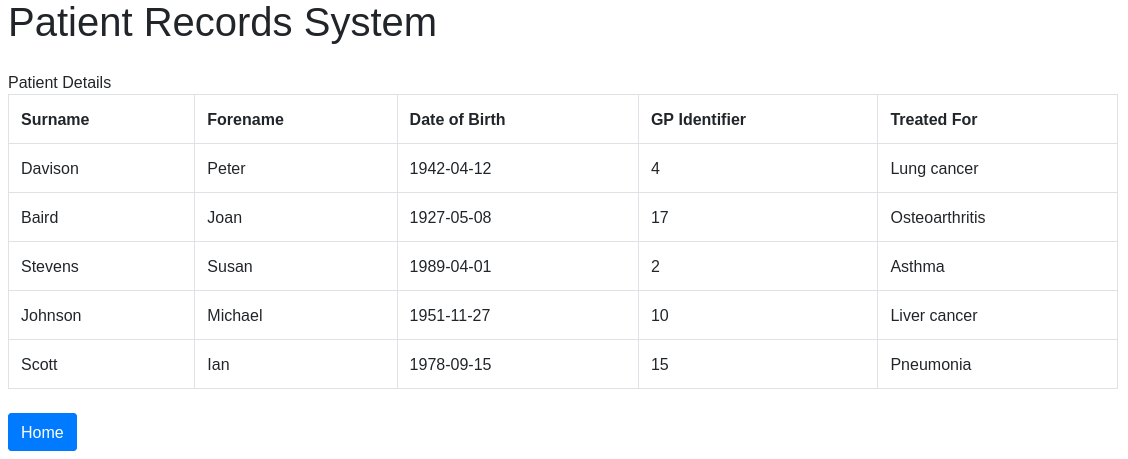
\includegraphics[width=\textwidth]{injection}
                \caption{Result of SQL injection to show all entries in the patients table}
                \label{injection}
            \end{figure}

            This vulnerability was discovered by looking at the source code.
            The queries at the top have \texttt{\%s} placeholders instead of
            \texttt{?} placeholders and are later used in a simple
            \texttt{String.format} operation. Finally, the surname parameter is
            passed verbatim from the request without validation or any scaping.
            This is a textbook example of an SQL injection and very easy to
            find.

            The injection in the authentication fields was found and exploited
            the same way.

        \subsection{Passwords in plaintext}
            % under which you should describe the nature of the flaw and how
            % you discovered it, providing examples or evidence where appropriate

            Storing passwords in plaintext is a vulnerability with very low
            visibility but high severity. External security validation tests
            will not detect it as a moderately secure application will not
            expose any details about the choice of data storage to the outside
            world. As this is considered an implementation detail, password
            storage policies are not normally made public either. They are also
            not considered as a feature by normal user and therefore not
            advertised. It may only be of interest to tech focused people but
            even then is rarely publicied. Due to most applications being
            closed source, indedepndent validation of the storage mechanism is
            not possible either.

            Plaintext storage is of high severity in the event of a data
            breach. When this happens, users do not only have their account
            with the breached service compromised. Instead, all accounts that
            share a password with that service are at high risk of authorised
            access. Users tend to frequently reuse passwords despite the best
            advice of industry proffesionals, which is most problematic in the
            event of data breaches. Changing the password in all instances
            where the password is shared is bound to leave some out. And even
            the best defences against data breaches occasionally fail so
            mitigating their impact is of utmost importance. Further, since
            password dumps are a frequent occurance, password dictionaries are
            readily available and releasing more samples only furthers the
            reduction of overall password effectiveness.

            The flaw was discovered by manually inspecting the database and the
            servlet souce code. Performing a \texttt{select * from user;} quer
            yields a full list of registered users and their plaintext
            passwords. Further, the source code performs filtering based on the
            plain password without any transformations. For example, user "Mary
            Jones" with a username of "mjones" has the password "marymary".


    \section{Fixes implemented}
        % Write a short (maximum of one A4 page) summary of the changes that
        % you have made, explaining in each case how it has fixed the problem

        \subsection{SQL injection}

            The fix is simple - replace the \texttt{java.sql.Statement}s with
            \texttt{java.sql.PreparedStatemt}s. To do this, the query templates
            need to have their \texttt{\%s} replaced with a \texttt{?} and then
            have them initialised at startup. Now instead of formatting the
            strings directly, the user input is given to the prepared statement
            with \texttt{setString} and executed and handled as before. This
            has to be done in both the \texttt{authenticated()} and
            \texttt{searchResults()} methods.

            This fixes the vulnerability because the unvalidated user input is
            no longer formatted into the query. Instead, the query is sent to
            the database at application initialision which returns a compiled
            version which is used to handle requests in its place. This way the
            user input is never part of the query itself but is rather sent as
            a parameter to the precompiled qeuery separately. Further, since
            the statement is precompiled, there is no way for a text based
            attack (but not others like the compiled format).


        \subsection{Hashed passwords}

            Again, the fix is simple - edit the database in place and replace
            the plaintext passwords with their base64 encoded SHA-256 digests,
            extending the size of the password field in the proces (to 44
            symbols) and adding a small salt field. Then, implement a simple
            \texttt{passHash()} method to calculate the hash of a string and
            use it in the \texttt{authenticated()} method to calculate the
            hashed plaintext password with its salt concatenation. That value
            is then compared to the hash which is stored in the database.

            This fixes the vulnerability since obtaining a source text for a
            hash is a very computationally expesive process. This way even if
            the user reused the password with other services, that plaintext is
            not know and therefore those services remain secure even in the
            event of a leak. Furhter, in case the service computes the hash
            locally and transmits that over the network, the salt value ensures
            that the leaked hash value is different to that another service
            might be storing. In effect, this prevents hash dictionary attacks.

\end{document}
